% !TEX root = ../../thesis.tex

\section{Intertext UIDL} \label{intertextUIDL}

Intertext UIDL (IUIDL) is an XML-based markup language that can be used to describe user interfaces. It features a layout system and UI components that could be used together as building blocks to put together a user interface. IUIDL is meant to be served from a generic backend, assembled on the backend based on the application logic. It is designed to be unopinionated, as it does not restrict how you assemble them or where you serve them from. For instance, below is an example Todo list. The Todo items are served from a Node.js server that uses Express.js framework, as it can be seen in Figure \ref{fig:todos_js}. The endpoint \textit{/todo} passes the Todo items to the Handlebar template

serves the render output of the template at 

\begin{figure}[H]
\begin{minipage}{\linewidth}
\begin{lstlisting}[language=javascript]
router.get('/todo', function(req, res, next) {

  const todos = [
    {
      title: 'Buy milk',
      done: false,
    },
    {
      title: 'Call mom',
      done: false,
    },
    {
      title: 'Prepare for presentation',
      done: true,
    },
  ];

  res.render('todo', {
    itemsToDo: todos.filter(item => !item.done),
    itemsDone: todos.filter(item => item.done),
  });
});
\end{lstlisting}
\end{minipage}
\caption{A simple Express endpoint that serves the render output of the Handlebars template at Figure \ref{fig:todos_template}}%
\label{fig:todos_js}%
\end{figure}


\begin{figure}[H]
\begin{minipage}{\linewidth}
\begin{lstlisting}[language=html]
<h3>To do ({{ itemsToDo.length }})</h3>

{{#each itemsToDo}}
  <block intent="default" flexDirection="row" alignItems="center" paddingLeft="4">
    <text flexGrow="1">{{this.title}}</text>
    <button intent="error">Remove</button>
    <button intent="success" marginLeft="2">Done</button>
  </block>
{{/each}}


<h3>Done ({{ itemsDone.length }})</h3>

{{#each itemsDone}}
  <block intent="default" flexDirection="row" alignItems="center" paddingLeft="4">
    <text flexGrow="1">{{this.title}}</text>
    <button intent="error">Remove</button>
    <button intent="success" marginLeft="2">Done</button>
  </block>
{{/each}}
\end{lstlisting}
\end{minipage}
\caption{Handlebars template that renders TODO items in IUIDL format}%
\label{fig:todos_template}%
\end{figure}


\begin{figure}[H]
  \centering
  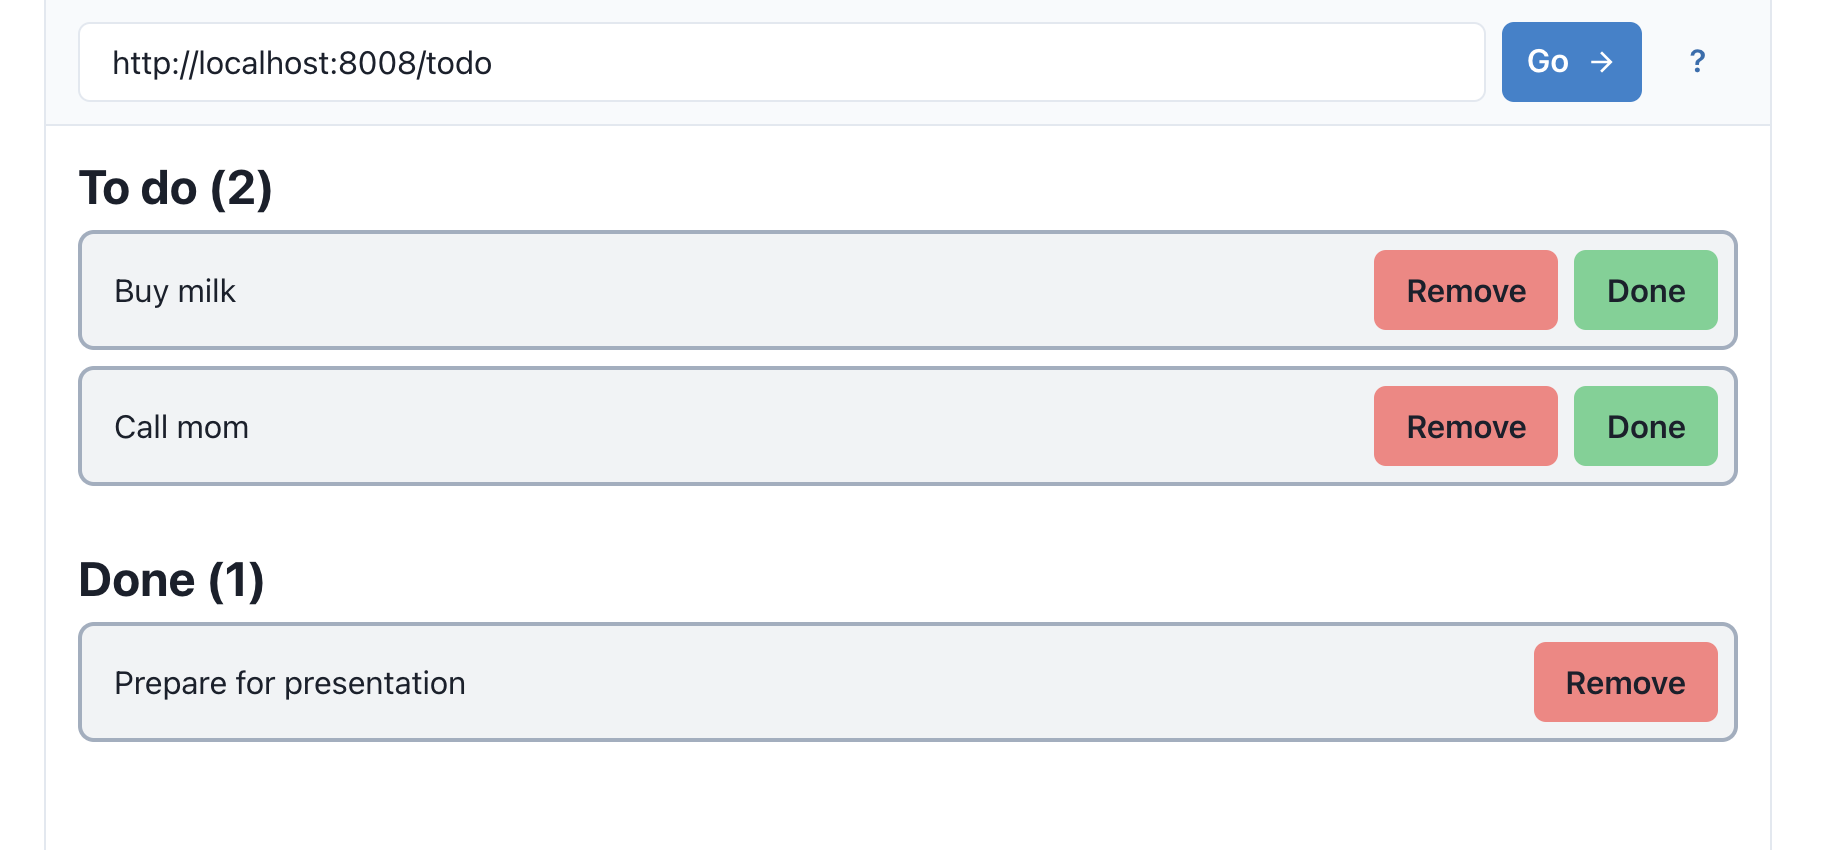
\includegraphics[width=13cm]{thesis/paper/images/todos.png}
  \caption{IUIDL served from the endpoint at Figure \ref{fig:todos_js} rendered on Intertext web client}%
  \label{fig:todos_output}%
\end{figure}



IUIDL is agnostic of the styling. 



Below is an example IUIDL code that generates 



% - intertext uidl
%   - terminologies? (platform-specific etc.)
%   - limitations? (<x.y>)
%   - json? xml?
 